% ================================================================
%  Suffix Trees & Ukkonen's Algorithm
% ================================================================

\section{Suffix Trees}

All the algorithms we have seen so far share a common pattern: we
\emph{preprocess the pattern}~$P$ and then scan the text~$T$ in a single
pass.
But what if the scenario is reversed?
Imagine a huge, mostly static text --- a genome, a legal corpus, or a
search-engine index --- that will be queried over and over with many
different patterns.
Preprocessing~$T$ \emph{once} so that each subsequent query can be
answered quickly is far more practical.

\aside{Think of it as building a ``phone book'' for every substring of $T$:
once built, any lookup takes time proportional to the query length, not
the text length.}

The data structure that achieves this is the \textbf{suffix tree}.
Its power comes from a simple observation: every substring of~$T$ is a
prefix of some suffix of~$T$.
So if we index \emph{all} suffixes, we can find any substring by walking
down from the root.

\subsection{Suffixes and Substrings}

\begin{observation}
  Let $T = t_1 t_2 \cdots t_n$.
  The set of substrings of $T$ equals the set of prefixes of all suffixes
  of $T$:
  \[
    \bigl\{\, T[i,j] \mid 1 \le i \le j \le n \,\bigr\}
    \;=\;
    \bigcup_{i=1}^{n}
    \bigl\{\,\text{prefixes of } T[i{,}] \,\bigr\}.
  \]
\end{observation}

This means a trie over all suffixes of $T$ encodes every substring.
Walking from the root following the characters of a query string~$Q$
either succeeds (meaning $Q$ is a substring of~$T$) or fails at some
point (meaning $Q$ does not occur in~$T$).

\subsection{Suffix Trie}

The first idea is the most direct one: build a trie that contains every
suffix of~$T$.

\begin{definition}[Suffix trie, $\mathrm{STrie}(T)$]
  \label{def:strie}
  Let $T = t_1 t_2 \cdots t_n$ be a string over an alphabet $\Sigma$.
  The \textbf{suffix trie} of~$T$, denoted $\mathrm{STrie}(T)$, is the
  (deterministic, acyclic) trie that accepts exactly the set $\sigma(T)$
  of all suffixes of~$T$ (including the empty string~$\varepsilon$).

  Formally, $\mathrm{STrie}(T) = (\mathcal{Q} \cup \{root, \bot\},\;
  \Sigma,\; g',\; f,\; root)$ where:
  \begin{itemize}[nosep]
    \item $\mathcal{Q}$ has one state for every distinct substring of~$T$.
    \item $g'(s,\, a)$ is the transition function: from state $s$
          (representing substring~$w$) reading character~$a$, go to the state
          representing~$wa$ (if $wa$ is a substring of~$T$).
    \item $f$ is the \textbf{suffix function}: $f(s)$ points to the state
          representing $w[2{,}]$ (i.e.\ $w$ with its first character removed).
          This is the exact analogue of the failure function in KMP /
          Aho--Corasick.
    \item $\bot$ is an auxiliary ``bottom'' state with
          $g'(\bot, a) = root$ for every $a \in \Sigma$, and
          $f(root) = \bot$.
  \end{itemize}
  The \textbf{final states} correspond to actual suffixes of~$T$
  (including $root = \varepsilon$).
\end{definition}

\aside{The suffix function $f$ is the direct analogue of KMP's failure
function: it links each state to its longest proper suffix that is still
a state.
The bottom state $\bot$ is a convenience --- it ensures that the
suffix-link chain starting from any state always terminates cleanly
at $\bot$, even when we fall off the root.}

\begin{example}[Suffix trie of $T = \texttt{cacao}$]
  \label{ex:strie-cacao}
  The suffixes of $\texttt{cacao}$ are:
  $\texttt{cacao}$, $\texttt{acao}$, $\texttt{cao}$, $\texttt{ao}$,
  $\texttt{o}$, and $\varepsilon$.

  The suffix trie $\mathrm{STrie}(\texttt{cacao})$ contains one state for every
  distinct substring: $\varepsilon$, \texttt{c}, \texttt{a}, \texttt{o},
  \texttt{ca}, \texttt{ac}, \texttt{ao}, \texttt{cac}, \texttt{aca},
  \texttt{cao}, \texttt{caca}, \texttt{acao}, \texttt{cacao},
  and so on --- a total of 16 states (including $root$).
  Figure~\ref{fig:strie-cacao} shows the structure.
\end{example}

\begin{figure}[H]
\centering
\begin{tikzpicture}[
  every node/.style={font=\small},
  state/.style={circle, draw=blue!50!black, fill=blue!6,
                minimum size=5mm, inner sep=0pt, font=\scriptsize},
  final/.style={state, double, double distance=1.2pt,
                draw=green!50!black, fill=green!6},
  edge label/.style={font=\scriptsize\ttfamily, text=gray!70!black},
  slink/.style={-Stealth, dashed, gray!45, thin, bend right=20},
]

% ── Level 0: root ─────────────────────
\node[state] (root) at (0,0) {$\varepsilon$};

% ── Level 1: single characters ────────
\node[state] (c)  at (-3.0,-1.5) {\texttt{c}};
\node[state] (a)  at ( 0.0,-1.5) {\texttt{a}};
\node[final] (o)  at ( 3.0,-1.5) {\texttt{o}};

\draw[-Stealth, thick] (root) -- (c)
  node[midway, above left, edge label] {c};
\draw[-Stealth, thick] (root) -- (a)
  node[midway, left, edge label] {a};
\draw[-Stealth, thick] (root) -- (o)
  node[midway, above right, edge label] {o};

% ── Level 2 ───────────────────────────
\node[state] (ca)  at (-4.2,-3.0) {\texttt{ca}};
\node[state] (ac)  at (-1.0,-3.0) {\texttt{ac}};
\node[final] (ao)  at ( 1.0,-3.0) {\texttt{ao}};

\draw[-Stealth, thick] (c) -- (ca)
  node[midway, above left, edge label] {a};
\draw[-Stealth, thick] (a) -- (ac)
  node[midway, left, edge label] {c};
\draw[-Stealth, thick] (a) -- (ao)
  node[midway, right, edge label] {o};

% ── Level 3 ───────────────────────────
\node[state] (cac) at (-5.4,-4.5) {\texttt{cac}};
\node[final] (cao) at (-3.0,-4.5) {\texttt{cao}};
\node[state] (aca) at (-1.0,-4.5) {\texttt{aca}};

\draw[-Stealth, thick] (ca) -- (cac)
  node[midway, above left, edge label] {c};
\draw[-Stealth, thick] (ca) -- (cao)
  node[midway, above right, edge label] {o};
\draw[-Stealth, thick] (ac) -- (aca)
  node[midway, left, edge label] {a};

% ── Level 4 ───────────────────────────
\node[state] (caca)  at (-6.0,-6.0) {\texttt{caca}};
\node[final] (acao)  at (-1.0,-6.0) {\texttt{acao}};

\draw[-Stealth, thick] (cac) -- (caca)
  node[midway, left, edge label] {a};
\draw[-Stealth, thick] (aca) -- (acao)
  node[midway, left, edge label] {o};

% ── Level 5 ───────────────────────────
\node[final] (cacao) at (-6.0,-7.5) {\texttt{cacao}};

\draw[-Stealth, thick] (caca) -- (cacao)
  node[midway, left, edge label] {o};

% ── Suffix links (only a few, for clarity) ────
\draw[slink] (ca)   to (a);
\draw[slink] (ac)   to (c);
\draw[slink] (cac)  to (ac);
\draw[slink] (aca)  to (ca);
\draw[slink] (cao)  to (ao);

\end{tikzpicture}
\caption{%
  Suffix trie $\mathrm{STrie}(\texttt{cacao})$.
  Solid arrows are transitions $g'(s,a)$; dashed arrows show selected
  suffix links $f(s)$.
  Double-bordered states are final (they correspond to actual suffixes).
  Every path from the root spells a distinct substring of
  $\texttt{cacao}$.
}
\label{fig:strie-cacao}
\end{figure}

\paragraph{The problem with suffix tries.}
The suffix trie is conceptually clean, but it is too large.
A string of length $n$ has $\Th{n^2}$ distinct substrings in the worst
case, so $\mathrm{STrie}(T)$ can have $\Th{n^2}$ states and $\Th{n^2}$
transitions.
Both building it and storing it takes $\Th{n^2}$ time and space --- the
same as explicitly listing all substrings.
We need a more compact representation.

\subsection{From Suffix Trie to Suffix Tree: Compaction}

\aside{The same idea that turns a trie into a \emph{Patricia trie} /
\emph{radix tree}: merge every chain of single-child internal nodes
into one edge with a multi-character label.}

Many states in the suffix trie have exactly one outgoing transition ---
they are just ``pass-through'' nodes on a single path.
If we merge every maximal chain of such single-child nodes into a single
edge (whose label is the concatenation of the individual character
labels), we obtain a much smaller tree.

\begin{definition}[Branching state, leaf, implicit state]
  A state of $\mathrm{STrie}(T)$ is:
  \begin{itemize}[nosep]
    \item a \textbf{branching state} if it has at least two outgoing
          transitions;
    \item a \textbf{leaf} if it has zero outgoing transitions
          (equivalently, it corresponds to a suffix that is not a proper
          prefix of another suffix);
    \item an \textbf{implicit state} otherwise (exactly one outgoing
          transition --- it sits in the interior of a compacted edge).
  \end{itemize}
  The root is always considered a branching state.
\end{definition}

\begin{definition}[Suffix tree, $\mathrm{STree}(T)$]
  \label{def:stree}
  The \textbf{suffix tree} of $T$ is the tree obtained from
  $\mathrm{STrie}(T)$ by keeping only the branching states and the
  leaves (the \textbf{explicit states}), and replacing every maximal
  chain of implicit states with a single edge.

  Each edge is labelled with a \emph{string} (not a single character).
  To avoid storing edge labels explicitly (which would again require
  $\Oh{n^2}$ space), we represent each label as a pair $(k, p)$ of
  positions in $T$: the label is $T[k \ldots p]$.

  The suffix tree $\mathrm{STree}(T)$ has:
  \begin{itemize}[nosep]
    \item at most $n$ leaves (one per suffix, exactly $n$ when a unique
          end-marker $\$$ is appended);
    \item at most $n-1$ internal branching nodes (by a standard tree
          argument);
    \item at most $2n - 1$ edges.
  \end{itemize}
  Hence $\mathrm{STree}(T)$ uses $\Oh{n}$ space.
\end{definition}

\aside{%
  By appending a special character
  $\$ \notin \Sigma$ to $T$, we guarantee
  that no suffix is a prefix of another.
  This makes every suffix end at a distinct leaf, so the tree
  has exactly $n+1$ leaves (counting $\$$).
}

\begin{figure}[H]
\centering
\begin{tikzpicture}[
  every node/.style={font=\small},
  state/.style={circle, draw=blue!50!black, fill=blue!6,
                minimum size=6mm, inner sep=0pt, font=\scriptsize},
  leaf/.style={circle, draw=green!50!black, fill=green!8,
               minimum size=6mm, inner sep=0pt, font=\scriptsize\bfseries},
  edge label/.style={font=\small\ttfamily, text=violet!60!black},
]

% ── Root ──────────────────────────────
\node[state] (root) at (0,0) {$\varepsilon$};

% ── Children of root ──────────────────
\node[state] (a)    at (-2.5,-2.0) {};
\node[leaf]  (o)    at ( 0.0,-2.0) {5};
\node[state] (c)    at ( 2.5,-2.0) {};

\draw[-Stealth, thick] (root) -- (a)
  node[midway, above left, edge label] {a};
\draw[-Stealth, thick] (root) -- (o)
  node[midway, left, edge label] {o};
\draw[-Stealth, thick] (root) -- (c)
  node[midway, above right, edge label] {c};

% ── Children of "a" node ─────────────
\node[leaf] (ao)   at (-4.0,-4.0) {4};
\node[leaf] (acao) at (-1.5,-4.0) {2};

\draw[-Stealth, thick] (a) -- (ao)
  node[midway, above left, edge label] {o};
\draw[-Stealth, thick] (a) -- (acao)
  node[midway, above right, edge label] {cao};

% ── Children of "c" node ─────────────
\node[leaf] (cao)   at ( 1.5,-4.0) {3};
\node[leaf] (cacao) at ( 4.0,-4.0) {1};

\draw[-Stealth, thick] (c) -- (cao)
  node[midway, above left, edge label] {o};
\draw[-Stealth, thick] (c) -- (cacao)
  node[midway, above right, edge label] {acao};

% ── Node labels ──────────────────────
\node[font=\tiny\sffamily, text=gray!55, below=1pt] at (a.south)
  {\textsf{a}};
\node[font=\tiny\sffamily, text=gray!55, below=1pt] at (c.south)
  {\textsf{ca}};

% ── Legend ────────────────────────────
\node[font=\scriptsize\sffamily, text=gray!50, anchor=north west]
  at (-5.5,-5.0) {
  Leaf labels = starting position of the suffix
};

\end{tikzpicture}
\caption{%
  Suffix tree $\mathrm{STree}(\texttt{cacao})$.
  Internal nodes correspond to branching states of the suffix trie;
  leaves are labelled with the starting position of the suffix they
  represent.
  Edge labels are substrings of $T$, stored as index pairs
  $(k, p)$ pointing into $T$ (shown here as the actual characters for
  readability).
  Compare with the suffix trie in Figure~\ref{fig:strie-cacao}: the
  $\Th{n^2}$ states have been compressed into $\Oh{n}$ nodes.
}
\label{fig:stree-cacao}
\end{figure}

\paragraph{Reference pairs.}
Since implicit states are not stored as nodes, we need a way to refer
to them.
A \textbf{reference pair} $(s, w)$ identifies an implicit (or explicit)
state by naming an explicit ancestor $s$ and the string $w$ that leads
from $s$ down to the desired state.
In practice, $w$ is stored as an index pair $(k, p)$ so that $w = T[k \ldots p]$.
When $w = \varepsilon$ (i.e.\ $k > p$), the reference pair
points to the explicit state $s$ itself.

A reference pair $(s, (k, p))$ is \textbf{canonical} if $s$ is the
closest explicit ancestor of the target state --- that is, the entire
string $T[k \ldots p]$ is consumed by a single edge or $s$ is the
state itself.
Canonizing a reference pair means ``walking down'' from $s$, consuming
full edges, until the remaining string fits within a single edge.

\subsection{Online Construction of the Suffix Trie}

Before tackling the linear-time suffix tree construction, it is
instructive to see how the suffix trie can be built \emph{online}
(left-to-right, one character at a time).
This na\"ive construction is $\Oh{n^2}$, but it introduces the key ideas
that Ukkonen's algorithm will later exploit.

\aside{``Online'' means: after reading $t_1 \ldots t_i$, the data
structure represents $\mathrm{STrie}(T^i)$ where
$T^i = t_1 \cdots t_i$.
We never look ahead at $t_{i+1}$.}

\paragraph{The key observation.}
Let $T^i = t_1 \cdots t_i$ denote the prefix of $T$ of length $i$.
The set of suffixes of $T^i$ can be obtained from the suffixes of
$T^{i-1}$ by appending $t_i$ to each one, plus the empty string:
\begin{equation}
  \label{eq:sigma-online}
  \boxed{\;\sigma(T^i) \;=\; \sigma(T^{i-1}) \cdot t_i
  \;\cup\; \{\varepsilon\}\;}
\end{equation}

\noindent
This is immediate: $T^i = T^{i-1} \cdot t_i$, so every suffix of $T^i$
is either $\varepsilon$ or has the form $\alpha \cdot t_i$ where
$\alpha$ is a suffix of $T^{i-1}$.

In terms of the trie, to go from $\mathrm{STrie}(T^{i-1})$ to
$\mathrm{STrie}(T^i)$ we need to extend every suffix of $T^{i-1}$
by the new character $t_i$.
This means adding a $t_i$-transition from each final state of
$\mathrm{STrie}(T^{i-1})$ that does not already have one.

\paragraph{The boundary path.}
The final states of $\mathrm{STrie}(T^{i-1})$ are exactly the
states representing the suffixes of $T^{i-1}$:
\[
  T^{i-1},\quad
  T^{i-1}[2{,}],\quad
  T^{i-1}[3{,}],\quad
  \ldots,\quad
  T^{i-1}[i{-}1{,}],\quad
  \varepsilon.
\]
These states are connected by the suffix function $f$:
$f(T^{i-1}) = T^{i-1}[2{,}]$,\;
$f(T^{i-1}[2{,}]) = T^{i-1}[3{,}]$,\; and so on down to
$f(\varepsilon) = \bot$.
This chain of suffix links is called the \textbf{boundary path} of
$\mathrm{STrie}(T^{i-1})$.

\begin{figure}[H]
\centering
\begin{tikzpicture}[
  every node/.style={font=\small},
  state/.style={rectangle, rounded corners=3pt, draw=blue!50!black, fill=blue!6,
                minimum height=6mm, inner sep=3pt, font=\small\ttfamily},
  bot/.style={rectangle, rounded corners=3pt, draw=gray!50, fill=gray!8,
              minimum height=6mm, inner sep=3pt, font=\small\sffamily},
  slink/.style={-Stealth, thick, red!50!black},
  newtr/.style={-Stealth, thick, green!50!black, dashed},
]

\node[state] (s1) at (0, 0)   {$T^{i-1}$};
\node[state] (s2) at (0,-1.4) {$T^{i-1}[2{,}]$};
\node[state] (s3) at (0,-2.8) {$T^{i-1}[3{,}]$};
\node        (dots) at (0,-3.8) {$\vdots$};
\node[state] (eps) at (0,-4.8) {$\varepsilon$};
\node[bot]   (bot) at (0,-6.2) {$\bot$};

\draw[slink] (s1) -- (s2) node[midway, right=4pt, font=\scriptsize\sffamily, text=red!50!black] {$f$};
\draw[slink] (s2) -- (s3) node[midway, right=4pt, font=\scriptsize\sffamily, text=red!50!black] {$f$};
\draw[slink] (s3) -- (dots);
\draw[slink] (dots) -- (eps);
\draw[slink] (eps) -- (bot) node[midway, right=4pt, font=\scriptsize\sffamily, text=red!50!black] {$f$};

% ── new t_i transitions ─────────────
\node[font=\scriptsize\sffamily, text=green!45!black, anchor=west]
  at (2.5,-0.0) {add $t_i$-transition?};
\node[font=\scriptsize\sffamily, text=green!45!black, anchor=west]
  at (2.5,-1.4) {add $t_i$-transition?};
\node[font=\scriptsize\sffamily, text=green!45!black, anchor=west]
  at (2.5,-2.8) {add $t_i$-transition?};

\draw[newtr] (s1.east) -- ++(1.8,0);
\draw[newtr] (s2.east) -- ++(1.8,0);
\draw[newtr] (s3.east) -- ++(1.8,0);

% ── brace: boundary path ────────────
\draw[decorate, decoration={brace, mirror, raise=8pt, amplitude=5pt},
      blue!40!black]
  (-1.2, 0.35) -- (-1.2,-6.55)
  node[midway, left=16pt, font=\footnotesize\sffamily, text=blue!40!black,
       align=center] {boundary\\path};

\end{tikzpicture}
\caption{%
  The boundary path of $\mathrm{STrie}(T^{i-1})$: the chain of
  suffix links from the deepest state $T^{i-1}$ down to $\bot$.
  To build $\mathrm{STrie}(T^i)$ we walk this path and add a
  $t_i$-transition from every state that does not already have one.
}
\label{fig:boundary-path}
\end{figure}

\paragraph{Active point and endpoint.}
When we walk down the boundary path from $T^{i-1}$ towards $\bot$,
at some point we hit a state that \emph{already} has a
$t_i$-transition.
Once we find such a state, \emph{all} states below it on the boundary
path also have a $t_i$-transition (because they represent shorter
suffixes, and if $\alpha \cdot t_i$ is a substring of $T^{i-1}$, then
so is every suffix of $\alpha$ followed by $t_i$).

\begin{definition}[Active point and endpoint]
  \label{def:active-endpoint}
  Let $s_1 = T^{i-1},\; s_2,\; \ldots,\; s_k = \varepsilon,\;
  s_{k+1} = \bot$ be the states on the boundary path.
  \begin{itemize}[nosep]
    \item The \textbf{active point} $s_j$ is the first state on the
          boundary path (from the top) that is \emph{not} a leaf.
    \item The \textbf{endpoint} $s_{j'}$ is the first state on the
          boundary path (from the top) that already has a
          $t_i$-transition (and is not a leaf).
  \end{itemize}
  The boundary path is thus partitioned into three zones:
  \begin{enumerate}[nosep]
    \item $s_1, \ldots, s_{j-1}$: leaves --- extending an existing
          branch (the $t_i$ is appended to the path leading to the leaf).
    \item $s_j, \ldots, s_{j'-1}$: non-leaf states without a
          $t_i$-transition --- a \emph{new branch} is created from each.
    \item $s_{j'}, \ldots, s_{k+1}$: states that already have a
          $t_i$-transition --- nothing to do.
  \end{enumerate}
\end{definition}

\begin{figure}[H]
\centering
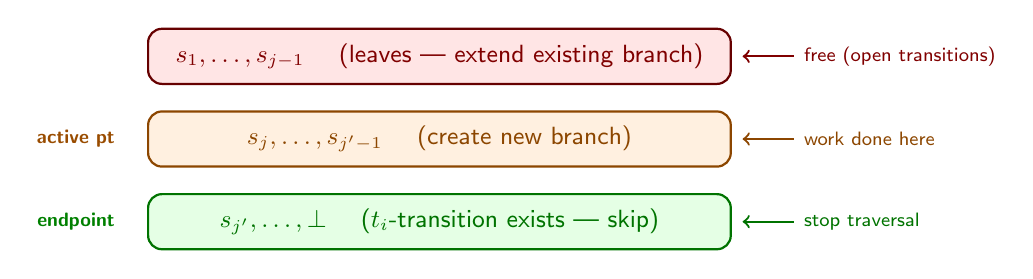
\begin{tikzpicture}[
  every node/.style={font=\small},
  zone/.style={rounded corners=5pt, thick},
]
\def\bw{7.4}
\def\bh{0.7}
\def\vgap{1.05}

% ── zone 1: leaves ──────────────────
\fill[red!10, zone] (0,0) rectangle (\bw, \bh);
\draw[red!40!black, zone] (0,0) rectangle (\bw, \bh);
\node[font=\small\sffamily, text=red!50!black] at (\bw/2, \bh/2)
  {$s_1, \ldots, s_{j-1}$ \quad (leaves --- extend existing branch)};

% ── zone 2: new branches ────────────
\fill[orange!12, zone] (0,-\vgap) rectangle (\bw, -\vgap+\bh);
\draw[orange!55!black, zone] (0,-\vgap) rectangle (\bw, -\vgap+\bh);
\node[font=\small\sffamily, text=orange!55!black] at (\bw/2, -\vgap+\bh/2)
  {$s_j, \ldots, s_{j'-1}$ \quad (create new branch)};

% ── zone 3: already done ────────────
\fill[green!10, zone] (0,-2*\vgap) rectangle (\bw, -2*\vgap+\bh);
\draw[green!45!black, zone] (0,-2*\vgap) rectangle (\bw, -2*\vgap+\bh);
\node[font=\small\sffamily, text=green!45!black] at (\bw/2, -2*\vgap+\bh/2)
  {$s_{j'}, \ldots, \bot$ \quad ($t_i$-transition exists --- skip)};

% ── right-side labels ──────────────────────────
\draw[<-, thick, red!50!black]
  (\bw+0.15, \bh/2) -- (\bw+0.8, \bh/2)
  node[right, font=\scriptsize\sffamily] {free (open transitions)};
\draw[<-, thick, orange!55!black]
  (\bw+0.15, -\vgap+\bh/2) -- (\bw+0.8, -\vgap+\bh/2)
  node[right, font=\scriptsize\sffamily] {work done here};
\draw[<-, thick, green!45!black]
  (\bw+0.15, -2*\vgap+\bh/2) -- (\bw+0.8, -2*\vgap+\bh/2)
  node[right, font=\scriptsize\sffamily] {stop traversal};

% ── left-side labels (active point / endpoint) ──
\node[font=\scriptsize\sffamily\bfseries, text=orange!60!black,
      anchor=east]
  at (-0.3, -\vgap+\bh/2) {active pt};
\node[font=\scriptsize\sffamily\bfseries, text=green!50!black,
      anchor=east]
  at (-0.3, -2*\vgap+\bh/2) {endpoint};

\end{tikzpicture}
\caption{%
  Partition of the boundary path into three zones when adding
  character $t_i$.
}
\label{fig:boundary-zones}
\end{figure}

\paragraph{Algorithm 1 (suffix trie, quadratic).}
The online construction of $\mathrm{STrie}(T)$ proceeds as follows:
start with $\mathrm{STrie}(\varepsilon)$ (just the root and $\bot$),
and for each character $t_i$ ($i = 1, \ldots, n$), walk down the
boundary path from the deepest state, creating new $t_i$-transitions
until we reach a state that already has one.

\begin{algorithm}[H]
  \caption{Online construction of $\mathrm{STrie}(T)$ (quadratic)}
  \label{alg:strie-quadratic}
  \KwIn{String $T = t_1 \cdots t_n$}
  \KwOut{$\mathrm{STrie}(T)$}
  create \textit{root} and $\bot$\;
  $f(root) \gets \bot$\;
  \For{every $a \in \Sigma$}{
    $g'(\bot, a) \gets root$\;
  }
  $r \gets root$ \tcp*{$r$ = deepest state on boundary path}
  \For{$i \gets 1$ \KwTo $n$}{
    $top \gets r$\tcp*{save current deepest state}
    \tcp{Walk boundary path from $top$ towards $\bot$}
    \While{$g'(r, t_i)$ is undefined}{
      create new state $r'$ and new transition $g'(r, t_i) = r'$\;
      \If{$r \neq top$}{
        $f(oldr) \gets r'$\tcp*{suffix link from previous new state}
      }
      $oldr \gets r'$\;
      $r \gets f(r)$\;
    }
    $f(oldr) \gets g'(r, t_i)$\;
    $r \gets g'(top, t_i)$ \tcp*{new deepest state $= T^i$}
  }
\end{algorithm}

\begin{theorem}
  \label{thm:strie-quadratic}
  $\mathrm{STrie}(T)$ can be constructed on-line in time and space
  proportional to the size of $\mathrm{STrie}(T)$, which is
  $\Oh{|T|^2}$ in the worst case.
\end{theorem}

\begin{proof}
  Each iteration $i$ traverses at most $i$ states on the boundary path,
  performing $\Oh{1}$ work per state (creating a new state, setting a
  suffix link, and following one suffix link).
  The total work is $\sum_{i=1}^{n} \Oh{i} = \Oh{n^2}$.
  The number of states is bounded by the number of distinct substrings,
  which is at most $\binom{n+1}{2} + 1 = \Oh{n^2}$.
\end{proof}

\subsection{Ukkonen's Linear-Time Construction}

The quadratic construction above already contains the right algorithmic
skeleton.
To reach $\Oh{n}$ time we need three key observations, each eliminating
a source of redundant work.

\begin{intermezzo}{Three tricks for $\Oh{n}$}

\begin{enumerate}
  \item \textbf{Open transitions (leaves extend for free).}
        In the suffix \emph{tree}, a leaf edge is stored as $(k, \infty)$
        --- the right endpoint ``stays at infinity''.
        When we append $t_i$, the label of every existing leaf edge
        automatically grows by one character, because $\infty$ now
        covers one more position.
        This means the entire first zone of the boundary path
        (all the leaves) is updated \emph{implicitly}, at zero cost.

  \item \textbf{The endpoint only moves to the right.}
        After processing $t_i$, the endpoint either stays in the same
        place or moves deeper along the boundary path for the next step.
        This means we never need to re-traverse the states above the
        current active point --- the algorithm ``resumes where it left
        off'' across iterations.

  \item \textbf{Suffix links + canonize.}
        Following a suffix link and then canonizing the reference pair
        takes amortised $\Oh{1}$ time (the total canonize work over
        all iterations is $\Oh{n}$).
\end{enumerate}
\end{intermezzo}

\paragraph{Open transitions.}
This is perhaps the most elegant trick.
In the suffix trie, extending a leaf means physically adding a new
transition.
In the suffix tree, leaf edges are labelled $(k, \infty)$ (or in
practice, $(k, |T|)$ at the end), where $\infty$ means ``to the
current end of the string''.
When we append $t_i$ to $T$, the ``current end'' shifts from $i-1$ to
$i$, so \emph{every} leaf edge automatically extends by one character,
without us touching it.

\aside{Open transitions eliminate the need to explicitly update
leaves: the first zone of the boundary path (Definition~\ref{def:active-endpoint})
costs $\Oh{0}$ per step instead of $\Oh{j-1}$.}

This means that once a leaf is created, it will \emph{never} need to
be revisited --- it extends passively with every new character.
The algorithm only needs to handle the second zone (creating new
branches) and detect when to stop (the third zone).

\paragraph{The procedures.}
Ukkonen's algorithm maintains a \emph{reference pair} $(s, (k, i-1))$
for the \textbf{active point}: the deepest non-leaf state on the
boundary path of $\mathrm{STree}(T^{i-1})$.
At each step $i$, three procedures cooperate:

\begin{description}[style=nextline, leftmargin=1.5cm]
  \item[\textsc{test-and-split}$(s, (k, p), t)$.]
    Tests whether the state with reference pair $(s, (k, p))$ already
    has a $t$-transition in the suffix tree.
    If $(s, (k,p))$ is an explicit state, it simply checks for a
    $t$-edge from $s$.
    If it is an implicit state (mid-edge), it checks whether the next
    character on the edge equals $t$.
    If not, it \textbf{splits} the edge, creating a new explicit
    branching node, and returns it.
    This is the analogue of the ``if there is no $t_i$-transition,
    create one'' step in Algorithm~\ref{alg:strie-quadratic}.

  \item[\textsc{canonize}$(s, (k, p))$.]
    Given a reference pair, walks down from explicit state $s$
    consuming full edges until the remaining string fits within a
    single edge.
    Returns the canonical pair $(s', (k', p))$ where $s'$ is as deep
    as possible.

  \item[\textsc{update}$(s, (k, i))$.]
    The main loop.
    Starting from the active point $(s, (k, i-1))$, it repeatedly
    calls \textsc{test-and-split} with the new character $t_i$.
    If a split occurs, a new leaf is created, a suffix link is set,
    and we follow the suffix link of $s$ to move to the next state on
    the boundary path (then \textsc{canonize}).
    The loop stops when \textsc{test-and-split} reports that a
    $t_i$-transition already exists (the endpoint has been reached).
\end{description}

\begin{algorithm}[H]
  \caption{\textsc{test-and-split}$(s, (k, p), t)$}
  \label{alg:test-and-split}
  \tcp{Returns (done?, explicit-state)}
  \If{$k \le p$}{
    let $g'(s, (k', p')) = s'$ be the $t_k$-transition from $s$\;
    \If{$t = t_{k' + p - k + 1}$}{
      \Return{$(\textbf{true},\; s)$}
    }
    \Else{
      create new state $r$\;
      replace transition: $g'(s, (k', k'+p-k)) = r$
        and $g'(r, (k'+p-k+1, p')) = s'$\;
      \Return{$(\textbf{false},\; r)$}
    }
  }
  \Else{
    \tcp{$(s, (k,p))$ is an explicit state (i.e.\ $s$ itself)}
    \If{there is no $t$-transition from $s$}{
      \Return{$(\textbf{false},\; s)$}
    }
    \Else{
      \Return{$(\textbf{true},\; s)$}
    }
  }
\end{algorithm}

\begin{algorithm}[H]
  \caption{\textsc{canonize}$(s, (k, p))$}
  \label{alg:canonize}
  \If{$p < k$}{
    \Return{$(s, (k, p))$}\tcp*{already canonical (empty string)}
  }
  find the $t_k$-transition $g'(s, (k', p')) = s'$ from $s$\;
  \While{$p' - k' \le p - k$}{
    $k \gets k + (p' - k') + 1$\;
    $s \gets s'$\;
    \If{$k \le p$}{
      find the $t_k$-transition $g'(s, (k', p')) = s'$ from $s$\;
    }
  }
  \Return{$(s, (k, p))$}
\end{algorithm}

\begin{algorithm}[H]
  \caption{\textsc{update}$(s, (k, i))$}
  \label{alg:update}
  \tcp{Returns the new active point reference pair}
  $oldr \gets root$\;
  $(\textit{done},\; r) \gets
    \textsc{test-and-split}(s, (k, i-1), t_i)$\;
  \While{\textbf{not} \textit{done}}{
    create new leaf $r'$ with transition
      $g'(r, (i, \infty)) = r'$\;
    \If{$oldr \neq root$}{
      create suffix link $f'(oldr) = r$\;
    }
    $oldr \gets r$\;
    $(s, k) \gets \textsc{canonize}(f'(s), (k, i-1))$\;
    $(\textit{done},\; r) \gets
      \textsc{test-and-split}(s, (k, i-1), t_i)$\;
  }
  \If{$oldr \neq root$}{
    $f'(oldr) = r$\tcp*{final suffix link}
  }
  \Return{$(s, k)$}
\end{algorithm}

\paragraph{The complete algorithm.}
Algorithm~\ref{alg:ukkonen} ties everything together.
It processes $T$ one character at a time, left to right.
After processing $t_i$, the data structure represents
$\mathrm{STree}(T^i)$.
The variable $(s, k)$ tracks the active point across iterations.

\begin{algorithm}[H]
  \caption{Ukkonen's on-line construction of $\mathrm{STree}(T)$}
  \label{alg:ukkonen}
  \KwIn{String $T = t_1 t_2 \cdots t_n\,\#$
        where $\#$ is a unique end-marker}
  \KwOut{$\mathrm{STree}(T)$}
  create \textit{root} and $\bot$\;
  \For{every $a \in \Sigma \cup \{\#\}$}{
    create transition $g'(\bot, (-j, -j)) = root$ for each $a = t_{-j}$\;
  }
  $f'(root) \gets \bot$\;
  $s \gets root;\quad k \gets 1;\quad i \gets 0$\;
  \While{$t_{i+1} \neq$ end of input}{
    $i \gets i + 1$\;
    $(s, k) \gets \textsc{update}(s, (k, i))$\;
    $(s, k) \gets \textsc{canonize}(s, (k, i))$\;
  }
\end{algorithm}

\subsection{Worked Example}

Let us trace Ukkonen's algorithm on $T = \texttt{cacao\$}$, the same
string from the paper.
We denote the characters $t_1 = \texttt{c}$, $t_2 = \texttt{a}$,
$t_3 = \texttt{c}$, $t_4 = \texttt{a}$, $t_5 = \texttt{o}$,
$t_6 = \texttt{\$}$.

\paragraph{Phase $i=1$ ($t_1 = \texttt{c}$).}
The tree is empty.
\textsc{update} calls \textsc{test-and-split} at the root: no
\texttt{c}-transition exists, so it creates a new leaf with edge
$(1, \infty)$ labelled \texttt{c\ldots}.
Follow the suffix link from \textit{root} to $\bot$;
$\bot$ always has a transition back to \textit{root}, so we stop.
Active point: $(root, 2)$ i.e.\ $(\textit{root},\, \varepsilon)$.

\begin{center}
\begin{tikzpicture}[
  state/.style={circle, draw=blue!50!black, fill=blue!6,
                minimum size=6mm, inner sep=0pt, font=\scriptsize},
  leaf/.style={circle, draw=green!50!black, fill=green!8,
               minimum size=5mm, inner sep=0pt, font=\scriptsize\bfseries},
  edge label/.style={font=\small\ttfamily, text=violet!60!black},
]
\node[state] (r) at (0,0) {$\varepsilon$};
\node[leaf]  (l1) at (0,-1.5) {1};
\draw[-Stealth, thick] (r) -- (l1)
  node[midway, right, edge label] {c\ldots};
\node[font=\scriptsize\sffamily, text=gray!55] at (1.8,0)
  {$\mathrm{STree}(\texttt{c})$};
\end{tikzpicture}
\end{center}

\paragraph{Phase $i=2$ ($t_2 = \texttt{a}$).}
Open transitions: leaf~1's edge $(1,\infty)$ now covers
\texttt{ca\ldots} --- no explicit work.
\textsc{update} from $(root, \varepsilon)$: root has no
\texttt{a}-transition, so create leaf~2 with edge $(2,\infty)$.
Follow suffix link to $\bot$, stop.

\begin{center}
\begin{tikzpicture}[
  state/.style={circle, draw=blue!50!black, fill=blue!6,
                minimum size=6mm, inner sep=0pt, font=\scriptsize},
  leaf/.style={circle, draw=green!50!black, fill=green!8,
               minimum size=5mm, inner sep=0pt, font=\scriptsize\bfseries},
  edge label/.style={font=\small\ttfamily, text=violet!60!black},
]
\node[state] (r) at (0,0) {$\varepsilon$};
\node[leaf]  (l1) at (-1.2,-1.5) {1};
\node[leaf]  (l2) at ( 1.2,-1.5) {2};
\draw[-Stealth, thick] (r) -- (l1)
  node[midway, left, edge label] {ca\ldots};
\draw[-Stealth, thick] (r) -- (l2)
  node[midway, right, edge label] {a\ldots};
\node[font=\scriptsize\sffamily, text=gray!55] at (2.5,0)
  {$\mathrm{STree}(\texttt{ca})$};
\end{tikzpicture}
\end{center}

\paragraph{Phase $i=3$ ($t_3 = \texttt{c}$).}
Open transitions: leaves~1 and~2 extend to cover \texttt{cac\ldots}
and \texttt{ac\ldots}.
\textsc{update} from $(root, \varepsilon)$: root already has a
\texttt{c}-transition (to leaf~1), so \textsc{test-and-split} returns
\textit{done} = true immediately.
\textbf{No new leaf is created.}
Active point becomes $(root, (3, 3))$, meaning we are now ``inside''
the edge to leaf~1, right after the \texttt{c}.

\aside{This is where the endpoint observation kicks in: the suffix
\texttt{c} already appears in the tree as a prefix of the existing edge,
so the construction pauses.
When a new character \emph{extends} an existing path in the tree
(``implicit extension''), no physical change is needed.}

The tree structure is unchanged from phase~2 (only the open transition
labels have grown).

\paragraph{Phase $i=4$ ($t_4 = \texttt{a}$).}
Open transitions: leaves grow to cover \texttt{caca\ldots} and
\texttt{aca\ldots}.
The active point is $(root, (3,3))$ = implicit state after
\texttt{c} on the root's \texttt{c}-edge.
\textsc{test-and-split} checks: the next character on that edge after
\texttt{c} is \texttt{a} --- and $t_4 = \texttt{a}$, so
\textit{done} = true.
No new node; active point advances to $(root, (3,4))$ (implicit state
for \texttt{ca}).

\paragraph{Phase $i=5$ ($t_5 = \texttt{o}$).}
Open transitions: leaves grow to \texttt{cacao\ldots} and
\texttt{acao\ldots}.
Active point is $(root, (3,4))$ = implicit state for \texttt{ca}.
\textsc{test-and-split}: the next character on the edge after
\texttt{ca} is \texttt{c} (since the edge spells
\texttt{cac\ldots}), but $t_5 = \texttt{o} \neq \texttt{c}$.
So we \textbf{split}: create a new internal node $v$ after
\texttt{ca}, with edges \texttt{cao\ldots} (leaf~1 continues) and
\texttt{o} (new leaf~3).
Then follow suffix link from $root$ to $\bot$... effectively the next
state to process is for the suffix \texttt{a}.
The active point for \texttt{a} is $(root, (4,4))$ = implicit state
on the \texttt{a}-edge.
\textsc{test-and-split} at that implicit state: next character
after \texttt{a} on that edge is \texttt{c}, but we need \texttt{o};
so split again: create internal node $w$ after \texttt{a}, with
edges \texttt{cao\ldots} (leaf~2 continues) and \texttt{o} (new leaf~4).
Set suffix link $f'(v) = w$.
Next state: $(root, \varepsilon)$, check \texttt{o} at root.
Root has no \texttt{o}-edge, so create leaf~5.
Set suffix link $f'(w) = root$.
Follow to $\bot$, stop.

\begin{center}
\begin{tikzpicture}[
  state/.style={circle, draw=blue!50!black, fill=blue!6,
                minimum size=6mm, inner sep=0pt, font=\scriptsize},
  leaf/.style={circle, draw=green!50!black, fill=green!8,
               minimum size=5mm, inner sep=0pt, font=\scriptsize\bfseries},
  edge label/.style={font=\small\ttfamily, text=violet!60!black},
  slink/.style={-Stealth, dashed, gray!45, thin, bend right=22},
]

\node[state] (r) at (0,0) {$\varepsilon$};

% ── from root ─────────────────────
\node[state] (ca) at (-3.0,-1.7) {};
\node[state] (a)  at ( 0.0,-1.7) {};
\node[leaf]  (l5) at ( 3.0,-1.7) {5};

\draw[-Stealth, thick] (r) -- (ca)
  node[midway, above left, edge label] {ca};
\draw[-Stealth, thick] (r) -- (a)
  node[midway, left, edge label] {a};
\draw[-Stealth, thick] (r) -- (l5)
  node[midway, above right, edge label] {o\ldots};

% ── from "ca" ─────────────────────
\node[leaf] (l1) at (-4.2,-3.5) {1};
\node[leaf] (l3) at (-1.8,-3.5) {3};

\draw[-Stealth, thick] (ca) -- (l1)
  node[midway, left, edge label] {cao\ldots};
\draw[-Stealth, thick] (ca) -- (l3)
  node[midway, right, edge label] {o\ldots};

% ── from "a" ──────────────────────
\node[leaf] (l2) at (-0.8,-3.5) {2};
\node[leaf] (l4) at ( 1.2,-3.5) {4};

\draw[-Stealth, thick] (a) -- (l2)
  node[midway, left, edge label] {cao\ldots};
\draw[-Stealth, thick] (a) -- (l4)
  node[midway, right, edge label] {o\ldots};

% ── suffix links ──────────────────
\draw[slink] (ca) to (a);

% ── labels ────────────────────────
\node[font=\tiny\sffamily, text=gray!55, below=0pt] at (ca.south)
  {\textsf{ca}};
\node[font=\tiny\sffamily, text=gray!55, below=0pt] at (a.south)
  {\textsf{a}};

\node[font=\scriptsize\sffamily, text=gray!55] at (4.5,0)
  {$\mathrm{STree}(\texttt{cacao})$};

\end{tikzpicture}
\end{center}

\paragraph{Phase $i=6$ ($t_6 = \texttt{\$}$).}
The end-marker $\$$ does not appear anywhere in the tree, so every
remaining suffix gets a new leaf.
After this phase, every suffix ends at its own leaf, and the
construction is complete.
The final tree is $\mathrm{STree}(\texttt{cacao\$})$.

\subsection{Complexity Analysis}

\begin{theorem}[Ukkonen, 1995]
  \label{thm:ukkonen-linear}
  Algorithm~\ref{alg:ukkonen} constructs the suffix tree
  $\mathrm{STree}(T)$ for a string $T = t_1 \cdots t_n$ on-line
  in $\Oh{n}$ time (assuming a constant-size alphabet or hash-based
  edge lookup).
\end{theorem}

\begin{formaldetails}[Proof of $\Oh{n}$ time]

We split the running time into two components and show each is $\Oh{n}$.

\paragraph{Component 1: everything except \textsc{canonize}.}
In each phase $i$, the \textbf{while} loop of \textsc{update}
(Algorithm~\ref{alg:update}) performs one iteration for each new leaf
created plus one final check that terminates the loop.
Each iteration does $\Oh{1}$ work (one call to \textsc{test-and-split}
with $\Oh{1}$ work, one leaf creation, one suffix link update, one
suffix link traversal).
The total number of leaves created across all $n$ phases is at most
$n$ (each suffix produces exactly one leaf).
The number of ``stop'' checks is also $n$ (one per phase).
So this component is $\Oh{n}$.

\paragraph{Component 2: \textsc{canonize}.}
The procedure \textsc{canonize}$(s, (k, p))$ walks down from
explicit state $s$, consuming edges of the suffix tree one by one.
Each edge consumed takes $\Oh{1}$ time (just compare the edge length
against $p - k + 1$ and follow the pointer).

To bound the total number of edges consumed by all calls to
\textsc{canonize} across the entire algorithm, we use an amortised
argument.
Define a potential function:
\[
  \Phi_i \;=\; \mathrm{depth}(s_i) - k_i + 1
\]
where $(s_i, k_i)$ is the active point reference pair after phase $i$,
and $\mathrm{depth}(s_i)$ is the string-depth (number of characters
from root to $s_i$) of the explicit state component.
Intuitively, $\Phi_i$ measures the ``amount of string'' in the
reference pair that is accounted for by explicit nodes rather than
by the remaining $(k, p)$ part.

\medskip
At each phase $i$:
\begin{itemize}[nosep]
  \item \textbf{The \textsc{update} loop} follows one suffix link per
        iteration.
        Following a suffix link from $s$ to $f'(s)$ decreases
        $\mathrm{depth}(s)$ by at least~1 (the suffix link target
        is one character shallower).
        Meanwhile, $k$ does not change during this step.
        So $\Phi$ decreases by at least~1.

  \item \textbf{Each \textsc{canonize} call} consumes edges, each of
        which increases $\mathrm{depth}(s)$ while also increasing $k$
        by the same amount.
        So each edge consumed leaves $\Phi$ unchanged.

  \item \textbf{The final \textsc{canonize}} (line~8 of
        Algorithm~\ref{alg:ukkonen}) moves $i$ from $i-1$ to $i$,
        which can increase $\Phi$ by at most~1 (the reference pair
        extends by one character).
\end{itemize}

Since $\Phi_0 = 0$, $\Phi_n \ge 0$, and each phase increases $\Phi$
by at most~1 while each suffix-link step decreases it by at least~1,
the total number of suffix-link steps (and hence the total number of
\textsc{canonize} edge-consumptions) is bounded by $n$.

\medskip
\textbf{Total:} both components are $\Oh{n}$, giving
$\Oh{n}$ overall.
\end{formaldetails}

\begin{remark}
  The ``on-line'' property is valuable in practice: we can build the
  suffix tree incrementally as characters arrive.
  After reading $t_1 \cdots t_i$, the tree already represents
  $\mathrm{STree}(T^i)$ and can answer queries about substrings
  of the text seen so far.
\end{remark}

\subsection{Applications of Suffix Trees}

Once $\mathrm{STree}(T)$ is built in $\Oh{n}$ time, many string
problems that would otherwise require specialised algorithms become
simple tree queries:

\begin{enumerate}[nosep]
  \item \textbf{Substring search.}
        Given a pattern $P$ of length $m$, walk down the tree following
        the characters of $P$.
        If we can spell out all of $P$, the subtree below that point
        contains all occurrences.
        Time: $\Oh{m + \text{occ}}$ where $\text{occ}$ is the number
        of occurrences.

  \item \textbf{Longest repeated substring.}
        The deepest internal node (by string-depth) corresponds to the
        longest substring that appears at least twice.
        A single DFS suffices.

  \item \textbf{Longest common substring of two strings.}
        Build $\mathrm{STree}(T_1 \$_1 T_2 \$_2)$ and find the
        deepest internal node that has leaves from both $T_1$ and $T_2$
        in its subtree.

  \item \textbf{Number of distinct substrings.}
        Sum the edge-label lengths over all edges: each edge contributes
        as many distinct substrings as its label length.
\end{enumerate}

\begin{observation}
  The suffix tree is the ``Swiss army knife'' of stringology: a single
  $\Oh{n}$-time preprocessing step unlocks $\Oh{m}$-time (or better)
  solutions to a wide family of substring problems.
\end{observation}
